% Chapter X

\chapter{Estensione del metodo alle linee ferroviarie}
\label{metodoLinee} % Chapter title
A partire dal metodo precendentemente descritto per gli edifici si è pensato di estendere il medesimo criterio anche alle rotte. Per rotta si intende una tratta che può essere una semplice strada, autostrata, o anche una linea ferroviaria sul quale bisogna effettuare lo studio di rischio frana alla quale potrebbe essere soggetta. Il metodo di base sviluppato per gli edifici calcolava il valore di exposure di determinati asset che erano riducibili a semplici punti geografici. Si deduce pertanto che l'estensione di tale metodo alle rotte richiede il campionamento di queste per approssimarle ad una serie di punti.
Prima di proseguire nel metodo bisogna definire alcune notazioni:

\begin{enumerate}
	\setcounter{enumi}{18}
	\item \textbf{$ \mathcal{R} $ (Routes)} $ = \{r_k(k=1,..,\mathbf{card}(\mathcal{R}) | r_k $ è una \textit{Route} ubicata all'interno dei confini della  GeoArea \}. Per \textit{Route} si intende una generica tratta (come ad esempio una ferrovia, un'autostrada) descritta dalla tupla < \textit{ID}, \textit{Name}, \textit{geometry}>. Il campo \textit{ID} identifica univocamente la tratta; \textit{Name} una sua etichetta nominale; \textit{geometry} rappresenta una geometria che descrive la tratta sul territorio. Nelle notazioni introdotte di seguito l'occorrenza del pedice $\{k\}$ viene usata $sempre$ per richiamare la \textit{Route} $k-esima$, ovvero alla tratta $r_k$ di $ \mathcal{R} $.
	
		\begin{figure}[h]
		\centering
		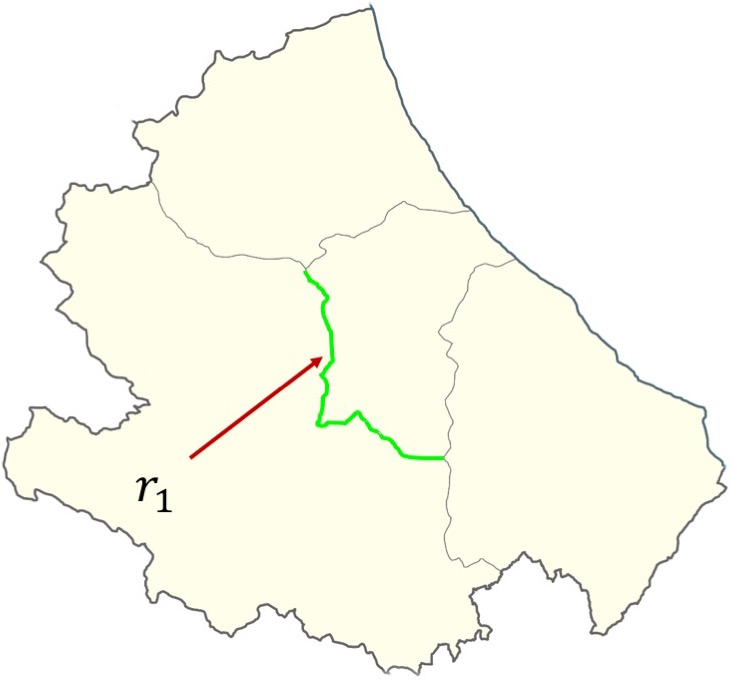
\includegraphics[width=0.4\textwidth]{images/routes1}
		\caption{la linea verde rappresenta la \textit{Route} $r_1$ dell'insieme $ \mathcal{R} $}
		\label{img:route}
		\end{figure}
	
	\item \textbf{$ \mathcal{RS}_k $ (Route Segments)} $ = \{rs_{k,s}(k=1,..,\mathbf{card}(\mathcal{R})),(s=1,..,\mathbf{card}(\mathcal{RS}_k))  | rs_{k,s} $ è una \textit{Route Segment} di una specifica \textit{Route} $r_k$ \}. Per \textit{Route Segment} $rs_{k,s}$ si intende la sotto-tratta $s-esima$ di lunghezza $v$ della \textit{Route} $r_k$. L'unione di tutti gli $rs_{k,s}$ restituisce l'elemento $r_k$. Nelle notazioni introdotte di seguito l'occorrenza del pedice $\{k,s\}$ viene usata $sempre$ per richiamare che ci si riferisce al \textit{Route Segment} $s-esimo$ della \textit{Route} $k-esima$.
		
	\item \textbf{$ \mathcal{RSP}_{k,s} $ (Route Segment Points)} $ = \{rsp_{k,s,p}(k=1,..,\mathbf{card}(\mathcal{R})),(s=1,..,\mathbf{card}(\mathcal{RS}_k)),(p=1,..,\mathbf{card}(\mathcal{RSP}_{k,s}))  | rsp_{k,s,p} $ è una \textit{Route Segment Point} di una specifica \textit{Route Segment} \}. Per \textit{Route Segment Point} $rsp_{k,s,p}$ si intende il $p-esimo$ punto ottenuto dal campionamento della \textit{Route Segment} $rs_{k,s}$. L'insieme di tutti gli $rsp_{k,s,p}$ con $k$ ed $s$ fissati, equivalgono all'inisieme di tutti i punti risultanti dal campionamento di $rs_{k,s}$.
	
\end{enumerate}

\noindent Il metodo consiste nel calcolare i valori di exposure delle \textit{Route Segments} di ogni \textit{Route} interna alla \textit{GeoArea}.
Il primo passo consiste nel "Segmentare" ogni tratta $r_k$ in sotto-tratte di lunghezza $v$ in modo da ottenerne:

\begin{equation}\label{eq:numerotratte}
m_{k}=\left\lceil\left(\frac{Lunghezza(r_k)}{v}\right)\right\rceil
\end{equation}
\\
Il numero $m_{k}$ di sotto-tratte è pari all'arrotondamento in eccesso tra il rapporto della lunghezza della tratta $r_k$ e il passo di segmentazione $v$. Si può intuire che tutte le sotto-tratte avranno lunghezza pari a $v$ eccetto l'ultima che avrà una lunghezza minore o al massimo uguale. Il valore di $m_k$ corrisponde pertanto alla $\mathbf{card}(\mathcal{RS}_{k})$
\\


	\begin{figure}[h]
	\centering
	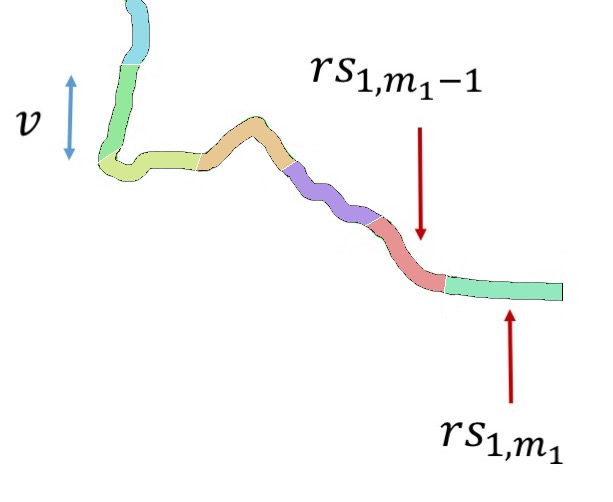
\includegraphics[width=0.4\textwidth]{images/routes2_new}
	\caption{Nella figura viene mostrata la procedura di segmentazione di una \textit{Route} in sotto-tratte di lunghezza $v$. Si può notare in questo caso che  l'ultima sotto-tratta $rs_{1,{m_1}}$ ha lunghezza inferiore a $v$}
	\label{img:segment}
	\end{figure}

\noindent A questo punto, ogni sotto-tratta $rs_{k,s}$ dovrà essere campionata ed approssimata ad una serie di punti. Si definisce pertanto un passo di campionamento $q << v$ che rappresenta la distanza massima tra i punti. Il numero di punti risultanti dal campionamento della sotto-tratta $rs_{k,s}$ sarà:

\begin{equation}\label{eq:numerotratte}
n_{k,s}=\left\lceil\left(\frac{Lunghezza(rs_{k,s})}{q}\right)\right\rceil
\end{equation}
\\
Al termine del campionamento, tutti i punti avranno una distanza dagli adiacenti pari al passo di campionamento ad eccezione dell'ultimo che avrà una distanza $\le q$ (Figura \ref{img:campionamento} e \ref{img:campionamento_2}). Pertanto si consiglia un passo di campionamento $q$ che sia divisibile per $v$ (in questo modo l'unico punto ad avere distanza $\le q$ dai vicini sarà l'ultimo punto della ultima sotto-tratta di $r_k$ ) Il valore di $n_{k,s}$ corrisponde alla $\mathbf{card}(\mathcal{RSP}_{k,s})$
\\

\begin{figure}[h]
	\centering
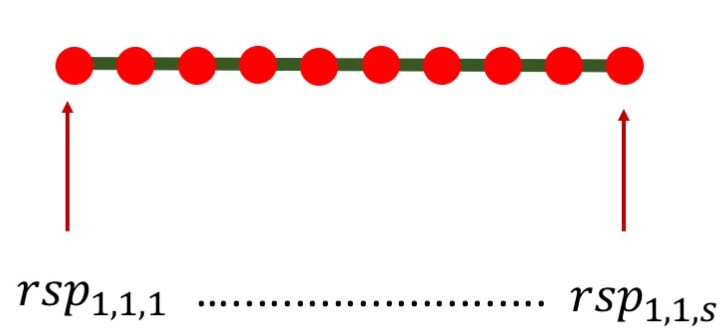
\includegraphics[width=0.6\textwidth]{images/routes3}
\caption{Esempio di campionamento di una \textit{Route Segment} con passo di campionamento $q$ (Caso con $v$ divisibile per $q$) }
\label{img:campionamento}
\end{figure}

\begin{figure}[h]
	\centering
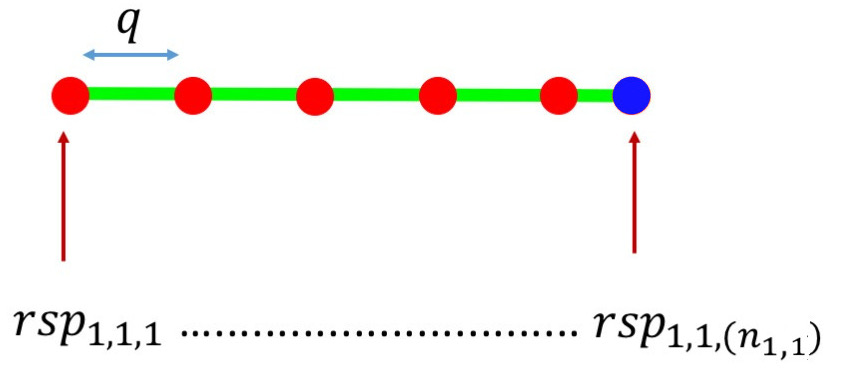
\includegraphics[width=0.6\textwidth]{images/routes4}
\caption{Esempio di campionamento di una \textit{Route Segment} con passo di campionamento $q$ (Caso con $v$ non divisibile per $q$). Si nota in questo caso l'ultimo punto di colore blue si trova a distanza <$q$ dall'adiacente }
\label{img:campionamento_2}
\end{figure}

\newpage
\noindent Una volta ottenuti i punti $rsp_{k,s,p}$ che approssimano la sotto-tratta $rs_{k,s}$, è possibile applicare il metodo base di calcolo per l'exposure. Per il metodo esteso alle tratte, si è deciso di lavorare su due sistemi diversi per la rappresentazione della exposure. Le definiamo con le seguenti notazioni:

\begin{enumerate}
\setcounter{enumi}{21}
\item \label{ERSP} \textbf{$ExpRSP$ (Exposure Route Segment Points)} =\\
$ \{exprsp_{k,s,p} (k=1,..,\mathbf{card}(\mathcal{R})),(s=1,..,\mathbf{card}(\mathcal{RS}_k)),(p=1,..,\mathbf{card}(\mathcal{RSP}_{k,s}))  | exprsp_{k,s,p} $ è il valore di \textit{exposure} del $p-esimo$ punto della sotto-tratta $rs_{k,s}$. Esso è descritto dalla tupla \textit{<ID,name,km,position,exposure>} ove \textit{ID} identifica univocamente il punto; \textit{name} rappresenta il nome della $r_k$ di appartenenza; \textit{km} identifica a quale sotto-tratta di $r_k$ ci si riferisce; \textit{position} rappresenta la posizione geografica di $rsp_{k,s,p}$; \textit{exposure} indica il valore di exposure del relativo punto.

\item \label{ERS} \textbf{$ExpRS$ (Exposure Route Segment)} =\\$ \{Exprs_{k,s} (k=1,..,\mathbf{card}(\mathcal{R})),(s=1,..,\mathbf{card}(\mathcal{RS}_k)) | exprs_{k,s} $ è il valore di \textit{exposure} della sotto-tratta $s-esima$ della tratta $r_k$. Esso è descritto dalla tupla \textit{<km,name,geometry,exposure>} ove \textit{km} identifica a quale sotto-tratta di $r_k$ ci si riferisce; \textit{name} rappresenta il nome della $r_k$ di appartenenza; \textit{geometry} rappresenta la geometria di $rs_{k,s}$, \textit{exposure} indica il valore di exposure della relativa sotto-tratta, intesa come sommatoria delle exposure dei punti $rsp_{k,s,p}$ della medesima. Ogni tupla è univocamente identificabile dalla coppia [km,name].

\end{enumerate}
\noindent Il primo sistema, rappresenta l'exposure per i singoli punti $rsp_{k,s,p}$ trattandoli come se fossero edifici $b_i$. Pertanto si applica lo stesso metodo del \textit{Capitolo 3} così da cacolare i valori di exposure per ogni punto. Infine tale risultato sarà rappresentato secondo la notazione \ref{ERSP}.
\bigbreak
\noindent Il secondo sistema invece parte dai risultati ottenuti dal primo ma ha l'obettivo di rappresentare l'exposure non per i singoli punti ma per le specifiche sotto-tratte $rs_{k,s}$. Il valore di exposure per singola sotto-tratta è data dalla seguente equazione:

\begin{equation}\label{eq:exprs}
exprs_{k,s}=\frac{1}{n_{k,s}}\left(\sum_{p=1}^{n_{k,s}} exprsp_{k,s,p}\right)
\end{equation}


\noindent Con parole esplicite, l'exposure di una sotto-tratta $rs_{k,s}$ equivale alla media delle exposure di tutti i punti $rsp_{k,s,p}$ ottenuti dal suo campionamento. Il risultato sarà rappresentato secondo la notazione \ref{ERS}.